\section{Experiments}
\label{sec:exp}
\textbf{Setup.} Each run is a complete rehearsal of the online phase on a local copy of the released simulator (sha256
pinned): 20 sequential calls of 50 points, starting from the training rows only. We compare
\emph{v1} (block descent with fixed class shares), \emph{v2} (v1 plus the training-derived shift bias), \emph{v4}
(v2 plus evidence-driven allocation) and the ablation \emph{v4j} (j for joint), which is v4 without the block
structure: every candidate moves all three buildings (each with its own move of the same class) from the incumbent
or a measured elite (one of the run's lowest-$R$ points), there are no base or combination points, and the plateau
filter and the re-application of improving coordinates are off because both need single-block results; the surrogate,
move classes, trust scale and posterior shares are unchanged. A variant with fewer late surrogate picks (v3) was
dropped after one run (107.78). The metric is the best $R$ after 20 calls. Different policies consume their random
streams differently, so seeds do not pair across policies, with one exception: the submitted policy h7 equals v4 for
calls 1--11 and pairs with it on its three seeds. We report mean $\pm$ standard deviation over seeds and an exact
two-sided permutation test on the difference of means.

\begin{table}[t]
\centering
\caption{Best $R$ (kWh) after 20 calls $\times$ 50 points on the real simulator. Call 10: mean best $R$ after call 10.
$p$: exact permutation test against v4. v4j also drops the plateau filter and coordinate re-application.
Reference: best training row 115.76, best offline submission 115.68. $^\ast$Seeds 7, 2026 and 11 only, where it
pairs with v4 (v4 mean 105.59).}
\label{tab:main}
\setlength{\tabcolsep}{2.6pt}
\begin{tabular}{lcccccc}
\toprule
Policy & $n$ & mean $\pm$ sd & min & max & call 10 & $p$\\
\midrule
v1: block descent & 3 & 106.89 $\pm$ 0.41 & 106.42 & 107.21 & 107.88 & 0.60\\
v2: + shift bias & 6 & 106.47 $\pm$ 0.93 & 105.11 & 107.49 & 107.38 & 0.76\\
\textbf{v4: + evidence slots} & 6 & \textbf{106.19 $\pm$ 1.78} & 103.28 & 108.05 & 107.12 & --\\
v4j: v4, joint moves & 6 & 107.84 $\pm$ 1.05 & 106.08 & 108.97 & 108.48 & 0.078\\
\midrule
h7 (submitted)$^\ast$ & 3 & 105.50 $\pm$ 2.52 & 102.81 & 107.81 & 107.00 & --\\
\bottomrule
\end{tabular}
\end{table}

\begin{figure}[t]
\centering
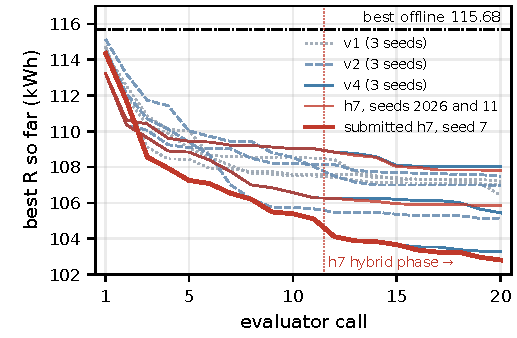
\includegraphics[width=\columnwidth]{figures/convergence.pdf}
\caption{Mean best measured $R$ per call; shaded: range over seeds. All values are simulator measurements.}
\label{fig:convergence}
\end{figure}

\textbf{RQ1: Does the block structure help?} Removing it, with the two rules that need it, and keeping everything
else raises the mean final $R$ from 106.19 to 107.84 ($+1.65$~kWh, $p=0.078$, six seeds each), and v4j trails v4 on
average from the second call on (mean after call 10: 108.48 vs.\ 107.12; Fig.~\ref{fig:convergence}). On its own, this
difference does not reach the 5\,\% level. v2 lacks the plateau filter and the re-application as well, so it isolates
the blocks from those two rules, though not from the posterior shares, the no-repeat rule or the eight call-1 jumps
(which never hit); it also beats v4j ($-1.37$~kWh, $p=0.041$). Among
the block-descent variants, neither the shift bias nor the allocation changes the final $R$ measurably (pairwise
$p\ge0.48$), so we also pool all 15 block-descent runs against v4j: $+1.40$~kWh for v4j, $p=0.024$. Both of these
comparisons were chosen after the primary one, so we read them as support, not proof. The mechanism is visible within these 15 runs. The combination step alone, i.e.\ the
gain of each new base over the previous incumbent before any new move is tried, accounts for 33.0\,\% of the total
descent. Its points beat the incumbent 83.7\,\% of the time, and the additive prediction~\eqref{eq:add} errs by a
median of $0.000$ and a mean absolute 0.17~kWh (59\,\% within 0.1), whereas surrogate picks land on average 3.54~kWh
above their prediction (mean absolute error 4.89) and hit 4.2\,\% of the time. In 43\,\% of calls, two or more
buildings improve in the same batch, so the composition is used, not only available. Without blocks, surrogate picks
miss by more (mean absolute error 7.08), because a joint move travels further from the data.

\begin{figure}[t]
\centering
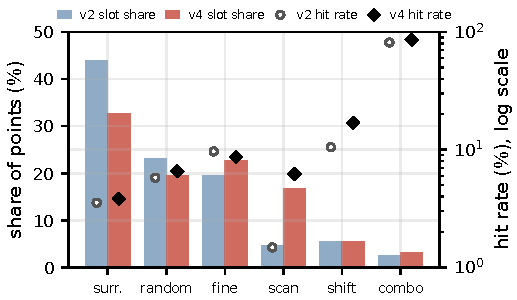
\includegraphics[width=\columnwidth]{figures/allocation.pdf}
\caption{Share of points (bars) and hit rate (markers) per move class, pooled over the seeds of v2 and v4. A hit is a
single-block point below its call's base, or a base or combination point (``combo'') below the previous incumbent.}
\label{fig:alloc}
\end{figure}

\textbf{RQ2: Does evidence-driven allocation help?} Not measurably. Over six seeds each, v4 and v2 end at 106.19
and 106.47 ($-0.28$~kWh, $p=0.76$). v4 leads at every call on average, but by at most 0.74~kWh (call~3), well within
the seed spread. The rules do what they were designed to do (Fig.~\ref{fig:alloc}): posterior shares move 11 points of
slot share from surrogate picks (44.0\,\% $\to$ 32.6\,\%; hit rate 3.8\,\% in v4) to scans (4.6\,\% $\to$ 16.7\,\%), whose
hit rate rises from 1.5\,\% to 6.2\,\% once they step outside detected plateaus. The extra hits, however, are small:
scans account for 7.0\,\% of v4's descent, and the share of late points (calls 11--20) that return an $R$ already
measured in the run, from a different weight vector, stays near 31\,\% (32.6\,\% in v2, 31.3\,\% in v4). Our first three seeds had suggested a gain of
0.93~kWh; three further seeds removed it.

\textbf{Other variants and the submitted policy.} Two attempts to avoid early commitment to one dominant objective
mix per building (vertex probes and parallel lanes) and a surrogate with fixed hyperparameters did not improve on v4
(means 106.26, 106.86 and 106.22 over three seeds, against 106.19). An independent whole-batch Bayesian optimisation with an additive
GP and 24,000 candidates per call reached 105.99 in its single run, level with v4's mean. The submitted h7 reaches
102.81 with the submitted seed; it is identical to v4 for calls 1--11 on each of its three seeds, so it pairs with v4
there, and the paired mean difference is $-0.09$ ($-0.47$, $-0.24$, $+0.43$), i.e.\ not distinguishable from v4.

\textbf{Reproducibility.} Recomputing the submitted run from its log reproduces all 20 batches exactly
(max $|\Delta W|=0$). Running the graded package on a second machine for two further seeds reproduced the $R$ of the 1,100 points
(2 seeds $\times$ 11 calls $\times$ 50) of calls 1--11 of the corresponding v4 rehearsals, which ran with a different harness on another machine, with
identical $R$ (four weight vectors differ in the last bit and two tied candidates swap places).
